\chapter{SAREF}
\label{cap:panoramicaSaref}
\section{Cos'è SAREF}

L'ontologia \textit{Smart Applications REFerence} (SAREF) è un'ontologia
condivisa che mira a fornire un modello di consenso per le applicazioni
intelligenti, consentendo il matching di asset esistenti in questo dominio.

SAREF si pone come obiettivo fornire una rappresentazione semantica condivisa
degli oggetti e dei servizi intelligenti, in modo che possano essere facilmente
condivisi, integrati e utilizzati tra diverse applicazioni.

All'interno di SAREF sono incluse 81 classi, 40 proprietà e 10 istanze,
utilizzabili per rappresentare ad esempio dispositivi IoT, attuatori, sensori,
edifici intelligenti, veicoli elettrici, etc..\\

SAREF si basa su quattro fondamenti:
\begin{itemize}
      \item Riutilizzo ed allineamento: progettato per essere riutilizzato in
            diverse applicazioni;
      \item Modularità: strutturato in moduli che permettono di utilizzare solo
            le parti dell'ontologia necessarie;
      \item Estensibilità: progettato per essere estendibile con nuovi moduli
            per
            esigenze specifiche;
      \item Manutenibilità: per facilitare il processo di identificazione e
            correzione di errori.
\end{itemize}

\subsection{SAREF overview}
Nella figura \ref{fig:saref} vengono identificate le principali classi e
relazioni che compongono l'ontologia.
\begin{figure}[!ht]
      \centering
      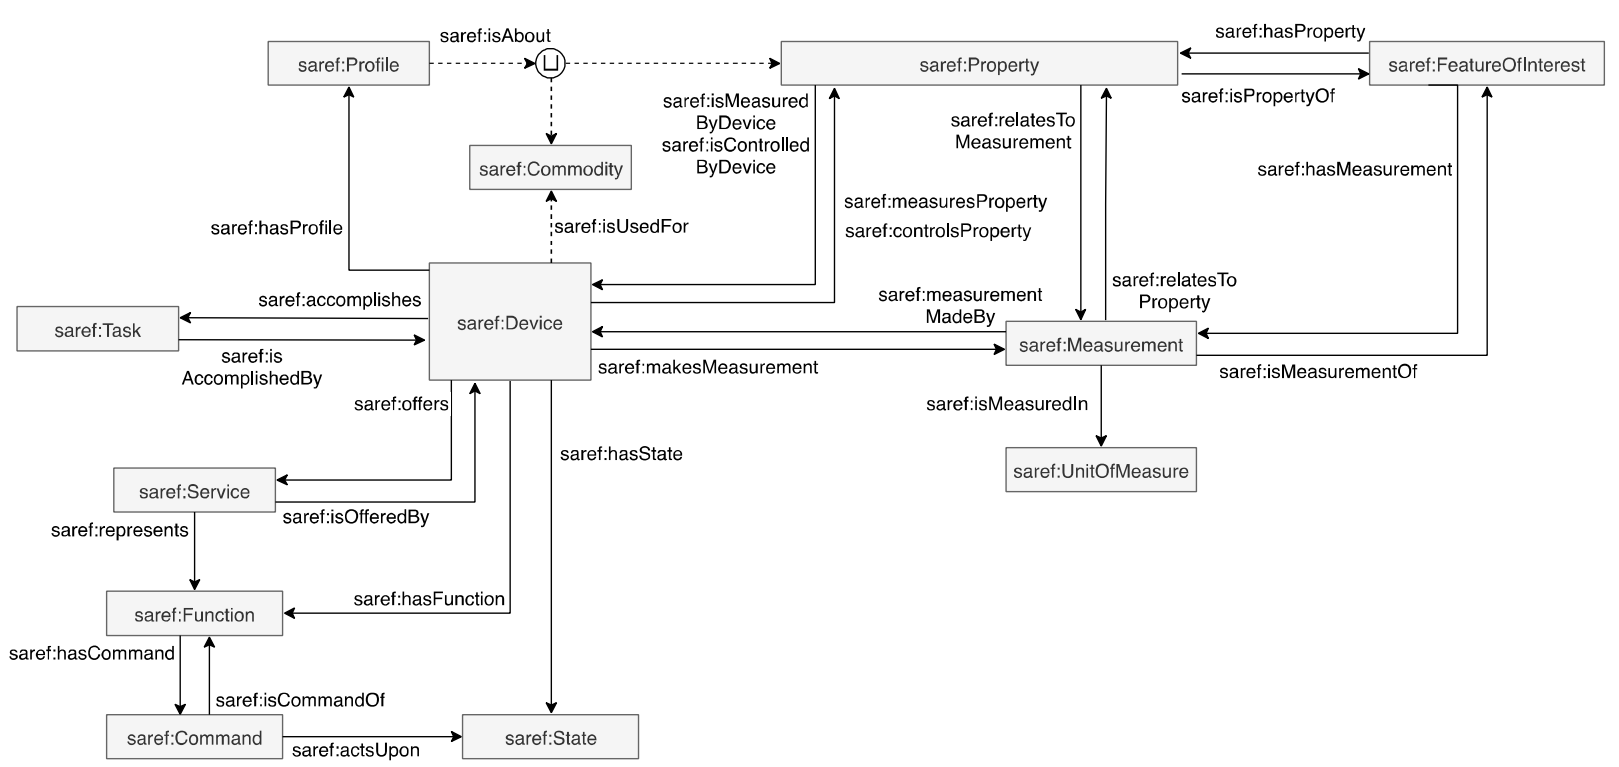
\includegraphics[width=13cm]{figures/saref.png}
      \caption{Classi e relazioni che compongono SAREF.}
      \label{fig:saref}
\end{figure}

L'entità principale è \texttt{saref:Device}, che rappresenta un dispositivo o
entità che ha le capacità di interagire con altri dispositivi o utenti. Ad essa
si collegano le altre classi dell'ontologia, tra cui: \texttt{saref:Task}, che
appresentare un'attività specifica che viene svolta da un dispositivo o da un
sistema, \texttt{saref:Service} che rappresenta un'istanza di un servizio
offerto,\texttt{saref:Property} che rappresenta una proprietà o un attributo di
un dispositivo o di un sistema.

I concetti rappresentati sono generici, rappresentando gli aspetti comuni di
contesti applicativi differenti ma sempre all'interno del dominio IoT. SAREF
può essere utilizzato in una vasta gamma di applicazioni intelligenti,
come ad esempio smart home, smart city, mobilità e trasporti, industria 4.0,
agricoltura intelligente ed altro.

\section{Estensioni di SAREF}
Per rappresentare al meglio i vari contesti nello specifico, sono state create
delle estensioni di SAREF.

Le estensioni rappresentano un insieme di ontologie specializzate, costruite a
partire dalla struttura di base di SAREF, ma con l'obiettivo di
modellare domini specifici come l'energia, l'edilizia, la città intelligente e
altri. Viene fornito un modello semantico comune per questi domini specifici,
in modo da poter rappresentare le informazioni in modo standardizzato e
interoperabile.
Inoltre, le estensioni di SAREF possono essere integrate con altre ontologie,
come l'InterConnect Ontology, per fornire una rappresentazione semantica comune
tra diverse ontologie e domini.

\subsection{SAREF4ENER}
L'estensione SAREF4ENER è stata creata per modellare gli aspetti specifici del
dominio dell'energia, come ad esempio i concetti di produzione, consumo,
generazione e gestione dell'energia elettrica.

Essa è stata sviluppata per fornire una rappresentazione comune e condivisa di
concetti relativi all'energia per facilitare l'interoperabilità tra sistemi
smart grid e i dispositivi connessi ad essi.

Inoltre, SAREF4ENER è stata progettata per essere compatibile con altre
ontologie utilizzate nel settore energetico, come l'ontologia Open Energy e
l'ontologia per i sistemi di stoccaggio dell'energia (Energy Storage System
Ontology), consentendo così l'interoperabilità tra diverse soluzioni
tecnologiche.

In sintesi, SAREF4ENER offre una solida base per la rappresentazione dei
concetti energetici e promuove l'interoperabilità tra sistemi, creando così
nuove opportunità per migliorare l'efficienza energetica, la sostenibilità e la
gestione intelligente dell'energia.\\

SAREF4ENER include 26 classi, 22 proprietà di oggetti e 10 proprietà di dati,
specificamente progettate per rappresentare concetti come la generazione e la
distribuzione di energia elettrica, il consumo energetico, la gestione delle
reti elettriche intelligenti, la misurazione dell'energia e altri concetti
chiave del settore energetico.

Questa estensione può essere utilizzata in diversi contesti, ad esempio nella
pianificazione energetica a livello comunale, nella gestione di microgriglie,
nella gestione di edifici intelligenti e nella gestione dell'energia domestica.

Nella figura \ref{fig:saref4ener} si può notare una panoramica di SAREF4ENER,
nella quale si differiscono le classi specifiche di SAREF4ENER che sono quelle
denotate da un cerchio arancione scuro, mentre le classi riutilizzate da altre
ontologie che sono quelle denotate da cerchi di color arancione chiaro.
\begin{figure}[!ht]
      \centering
      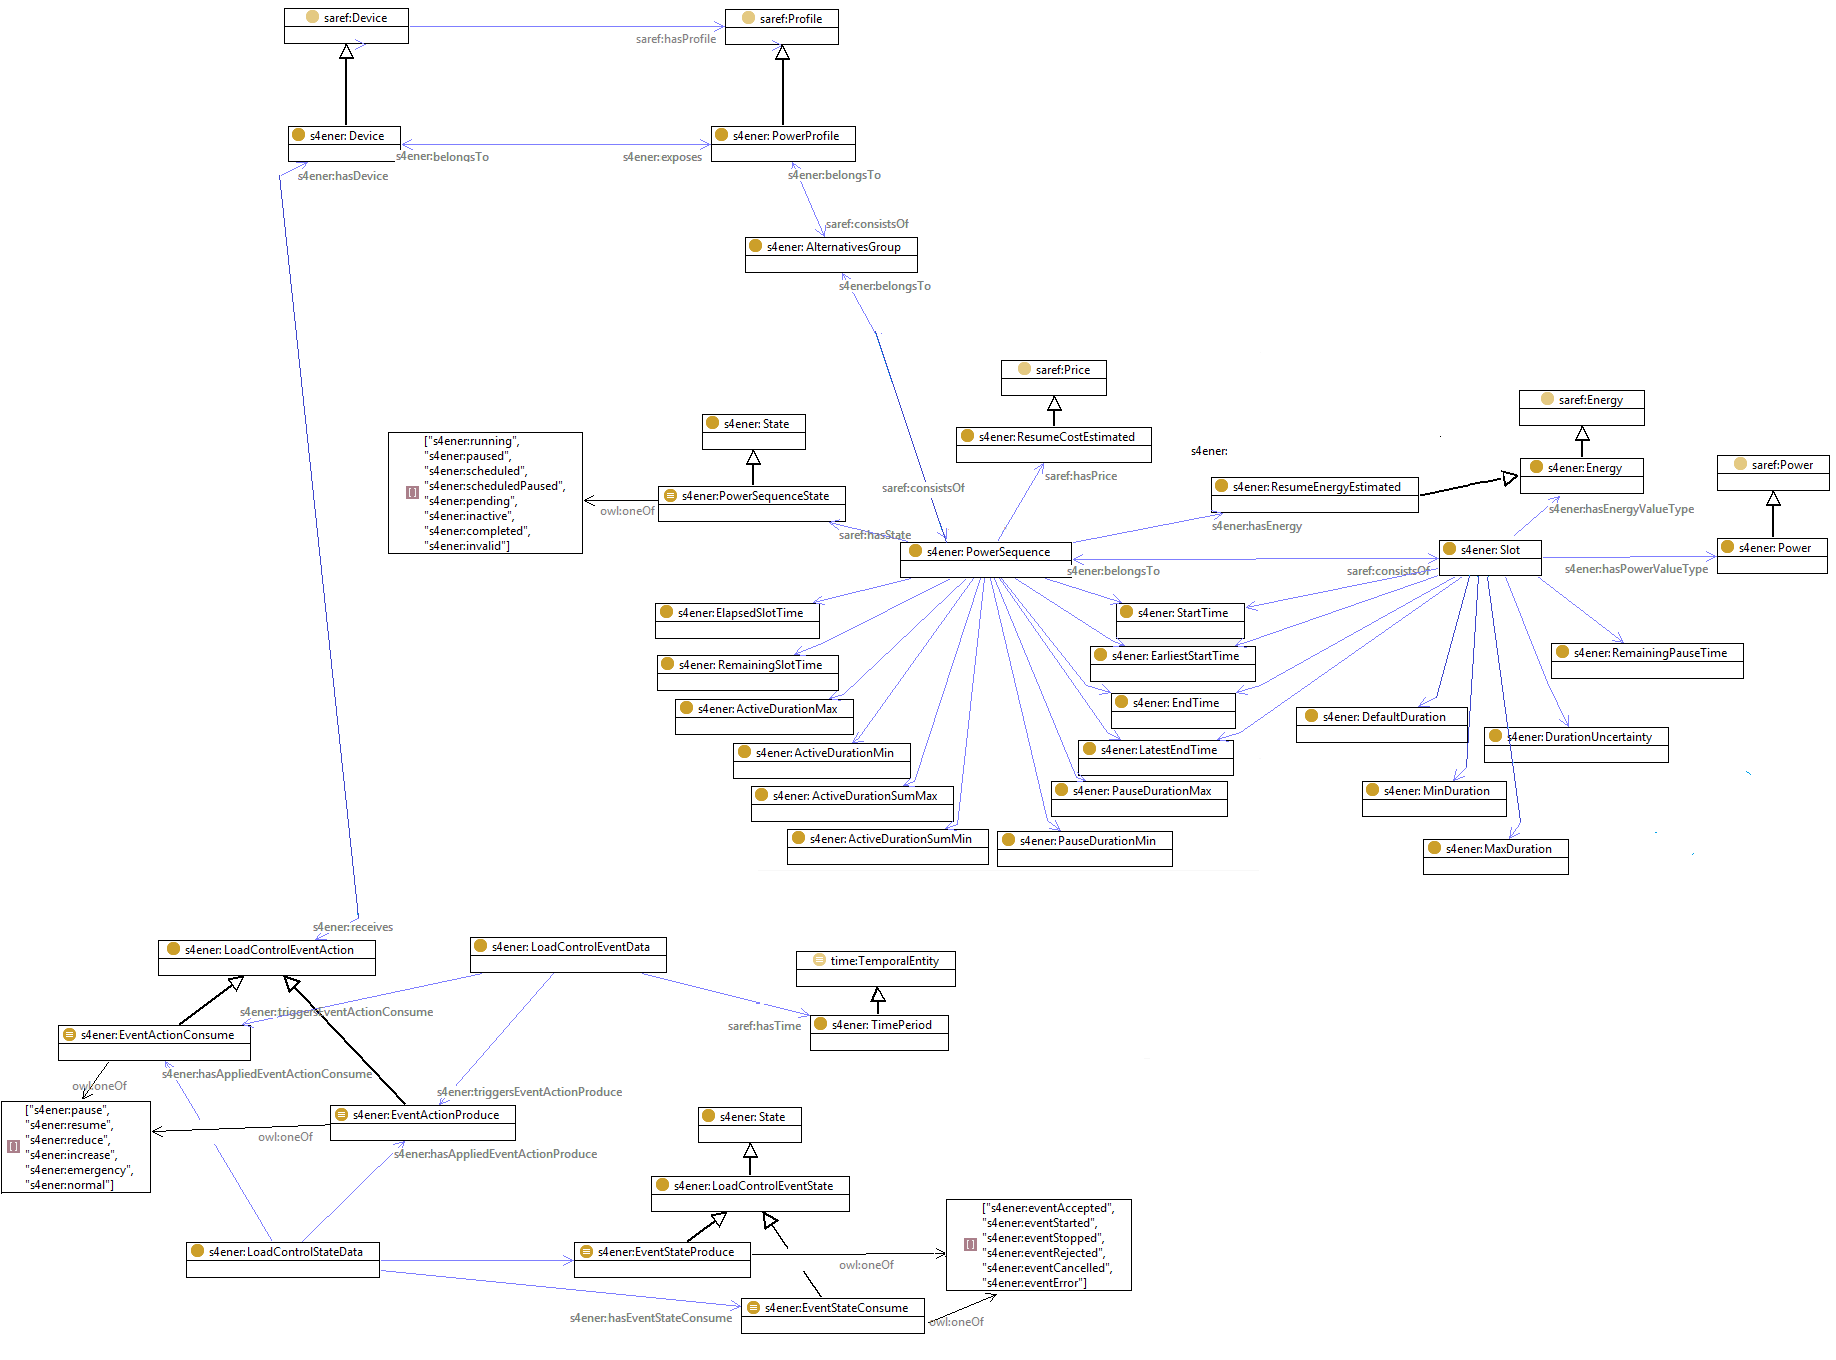
\includegraphics[width=15cm]{figures/saref4ener.png}
      \caption{Classi e relazioni che compongono SAREF4ENER.}
      \label{fig:saref4ener}
\end{figure}

Nelle entità presenti, quelle definite da SAREF4ENER hanno il prefisso
\texttt{s4ener}, mentre se è riutilizzato da un'altra ontologia è indicato nel
namespace.

Ci sono entità che vengono ereditate ed estese in maniera più specifica al
contesto, come ad esempio \texttt{Device} o \texttt{Profile}.
\texttt{PowerProfile} è una sottoclasse di \texttt{Profile}, che viene esposta
da un \texttt{Device}. \texttt{PowerProfile} consiste in uno o più
\texttt{AlternativesGroup} che a sua volta consiste in una o più
\texttt{PowerSequence}, composto anche esso da uno o più \texttt{Slot}.

\subsection{SAREF4BLDG}
SAREF4BLDG è un'estensione che si concentra sul dominio dell'edilizia,
e modella proprietà di edifici, come le proprietà degli impianti di
riscaldamento, la qualità dell'aria interna, l'illuminazione ed altre.

È stato creato basandosi sugli standard forniti da \textit{Industry Foundation
      Classes} (IFC) con le informazioni sulle costruzioni.

L'intero standard è stato trasformato siccome supera l'ambito dell'estensione,
che è limitata ai device ed alle applicazioni all'interno del dominio degli
edifici.

L'obiettivo di SAREF4BLDG è fornire un modello semantico condiviso per
descrivere gli edifici e le informazioni ad essi associate, al fine di
consentire l'interoperabilità tra i diversi sistemi e applicazioni che operano
nell'ambito dell'edilizia. Grazie a SAREF4BLDG, le informazioni sui singoli
componenti degli edifici possono essere facilmente integrate e scambiate tra
diversi sistemi, consentendo un controllo più efficiente e intelligente degli
edifici stessi.

Gli apparecchi intelligenti dei produttori che supportano il modello di dati
IFC possono comunicare facilmente tra loro utilizzando questa ontologia. Per
fare ciò, SAREF4BLDG dovrebbe essere utilizzato per annotare o generare
descrizioni di dispositivi neutri che possono essere condivisi tra le parti
interessate. Questa standardizzazione semantica dei dispositivi consente una
migliore interoperabilità e scambio di informazioni, creando quindi una base
per la creazione di servizi intelligenti per l'edilizia.

Attualmente però l'interoperabilità tra attori (come architetti, ingegneri e
produttori di componenti del prodotto) e applicazioni che gestiscono le
informazioni sull'edificio coinvolte nelle diverse fasi del ciclo di vita
dell'edificio, manca.

Essa definisce 72 classi, 179 tipi di oggetti e 82 proprietà di tipo dati, che
coprono le diverse informazioni relative all'edilizia.

L'ontologia SAREF ha generalizzato e trasferito la relazione tra spazi di
costruzione e dispositivi e oggetti di costruzione per consentire ai primi di
contenere entrambi i tipi di elementi. Pertanto, sia la classe
\texttt{BuildingObject} che \texttt{Device} sono state dichiarate come
sottoclassi
di \texttt{PhysicalObject}. Inoltre, la classe \texttt{BuildingDevice}
rappresenta
i dispositivi di costruzione ed è una sottoclasse di entrambe le classi
\texttt{Device} e \texttt{BuildingObject}.

Queste nozioni sono identificate nella figura \ref{fig:saref4bldg}.
\begin{figure}[!ht]
      \centering
      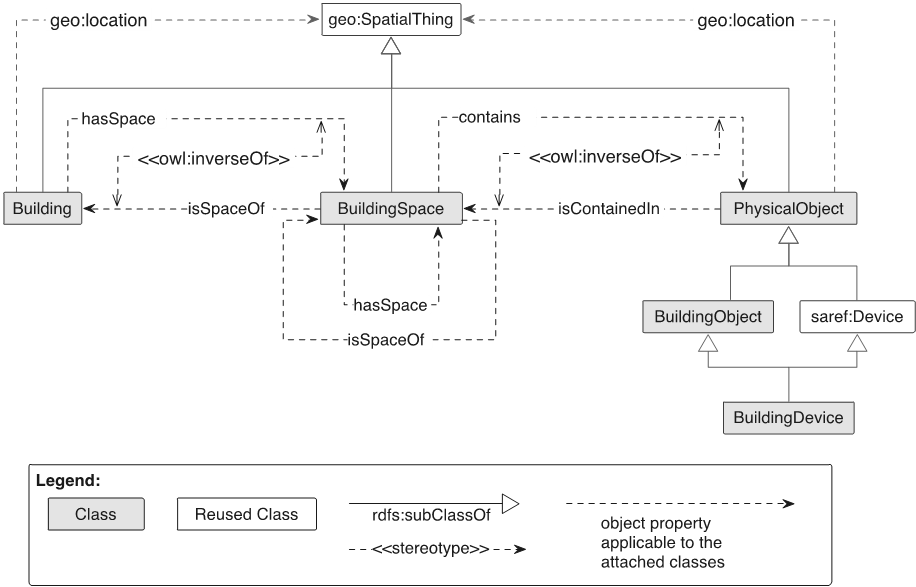
\includegraphics[width=13cm]{figures/saref4bldg.png}
      \caption{Classi e relazioni che compongono SAREF4BLDG.}
      \label{fig:saref4bldg}
\end{figure}

\subsection{SAREF4CITY}
SAREF4CITY è un'altra estensione di SAREF, che si focalizza sulla modellazione
di concetti specifici delle città intelligenti, come ad esempio la gestione del
traffico, la raccolta dei rifiuti, la sicurezza pubblica e così via, al fine di
supportare l'interoperabilità tra i dispositivi IoT intelligenti e i servizi
smart city. L'obiettivo di SAREF4CITY è quello di fornire una base comune di
informazioni semantiche per consentire la cooperazione tra i servizi
intelligenti delle città.

SAREF4CITY definisce un insieme di classi, proprietà e relazioni semantiche per
descrivere i concetti chiave delle città intelligenti, come ad esempio le
infrastrutture, le risorse, i servizi, gli eventi e i sensori.

Inoltre, SAREF4CITY è stato progettato per essere compatibile con altre
ontologie utilizzate nel contesto delle città intelligenti, come ad esempio
l'ontologia SSN (Semantic Sensor Network) per i sensori e l'ontologia CityGML
per la modellazione 3D degli edifici e delle città. Ciò consente di integrare
le informazioni provenienti da diverse fonti in un'unica base di conoscenza
comune e interoperabile.

Alcuni casi d'uso in questo caso potrebbero essere: eHealth, Smart Parking,
monitoraggio dell'aria e della mobilità.

Tenendo conto delle ontologie, dei modelli di dati, degli standard e dei set di
dati forniti dalle parti interessate identificate, una serie di requisiti è
stata identificata e raggruppata in categorie come topologia, area
amministrativa, oggetto della città, evento, misurazione, indicatore di
prestazioni chiave e servizio pubblico. Questi requisiti sono stati convalidati
durante il "SAREF4CITY Validation Workshop" alla IoT Week a Bilbao il 4 giugno
2018 e sono stati apportati dei cambiamenti in base ai feedback e ai risultati.
I requisiti identificati sono stati utilizzati come input per lo sviluppo
dell'ontologia, che è stata definita in modo modulare in base alle categorie
sopra menzionate.

SAREF4CITY comprende 31 classi, 36 proprietà degli oggetti e 7 proprietà del
tipo di dati. Molte delle classi e proprietà sono stati riutilizzati partendo
da altre ontologie come ad esempio SAREF. La figura \ref{fig:saref4city} mira a
mostrare una panoramica globale delle principali classi di SAREF4CITY e delle
loro relazioni reciproche.

\begin{figure}[!ht]
      \centering
      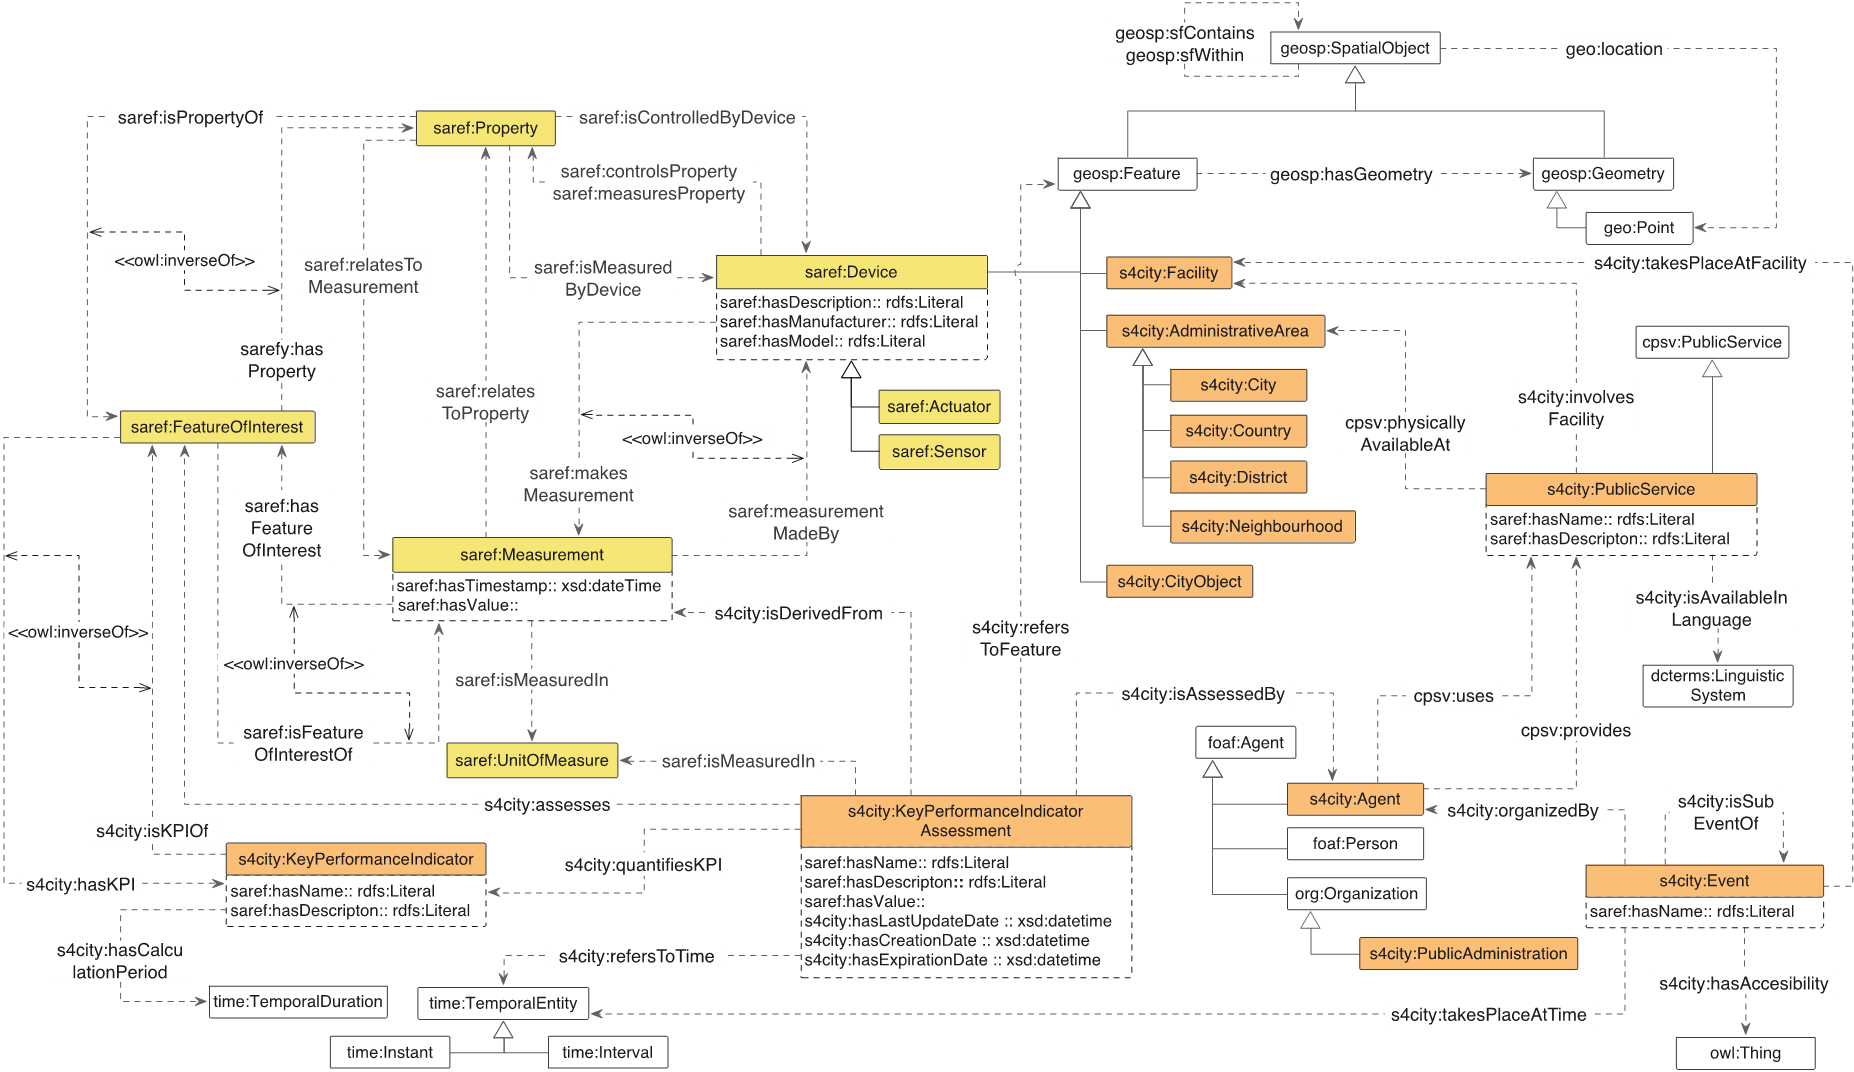
\includegraphics[width=13cm]{figures/saref4city.png}
      \caption{Classi e relazioni che compongono SAREF4CITY.}
      \label{fig:saref4city}
\end{figure}